\documentclass[a4paper, twoside]{article}

\usepackage{graphicx}
\usepackage{color}
\usepackage{multirow}
\usepackage{booktabs}

\usepackage{epsfig}
\usepackage{subfigure}
\usepackage{calc}
\usepackage{amssymb}
\usepackage{amstext}
\usepackage{amsmath}
\usepackage{amsthm}
\usepackage{multicol}
\usepackage{pslatex}
\usepackage{apalike}

\subfigtopskip=0pt
\subfigcapskip=0pt
\subfigbottomskip=0pt

\usepackage{siunitx}
\usepackage{tikz}

\usetikzlibrary{calc,arrows.meta,intersections,backgrounds,shapes.misc}

\usepackage{SCITEPRESS}     % Please add other packages that you may need BEFORE the SCITEPRESS.sty package.

\begin{document}

\title{Designing an Indoor Guidance System for the Visually Impaired} 

\author{
  \authorname{John Anon{\sup{1}}}
  \affiliation{\sup{1}Anon University of Anon, Anonville, Anonistan}
  \email{anon.anon@anon.com}
%\affiliation{\sup{1}Lincoln Centre for Autonomous Systems (L-CAS), University of Lincoln, Lincoln, UK}
%\email{jlock@lincoln.ac.uk}
}

\keywords{Active vision, vision impaired, Markov decision process, object search}

\abstract{In this work, we propose an active vision system that uses a Markov Decision Process and mobile phone to enable a user to find an object in an unknown environment. This project aims to deliver a workable system to the visually impaired, but a set of experiments were carried out with sighted participants to determine the effectiveness of the system. We found that the system works reasonably well and compares well to similar systems. However, some improvements are required before it is ready for real-world use. }

\onecolumn \maketitle \normalsize \vfill

\section{\uppercase{Introduction}}

\noindent We are designing an indoor navigation system targeted towards enabling blind and visually impaired (VI) users to safely safely navigate towards their desired destination or find an object in an unknown and dynamic environment. One requirement for this is the ability for a device to automatically make sense of the user's surroundings and determine the optimal route to get to the final destination based on what the user/camera sees, thereby roughly emulating a normally sighted user's navigation strategy in an unknown environment.

In this paper we discuss the first steps we've taken into implementing such a system. Specifically, we implemented a system with the capability to understand the user's surroundings and determine what the next best course of action is to reach the target location, based on what the system is currently seeing and what it has seen in the past. We used a Markov Decision Process (MDP)~\cite{bellman1957markovian} to produce a so-called policy that defines the optimal action, $a$, our agent (the guidance system in this case) takes when it is in some state $s$.  

This work's main contribution is the design of a guidance system and MDP that can drive a user to point a mobile device's camera towards a given point in space in and find a target object. The interface is pictured in Figure~\ref{fig:system-screenshot}. We also present and discuss preliminary experimental results to show how effective the system is at finding a target.

\begin{figure}
  \centering
  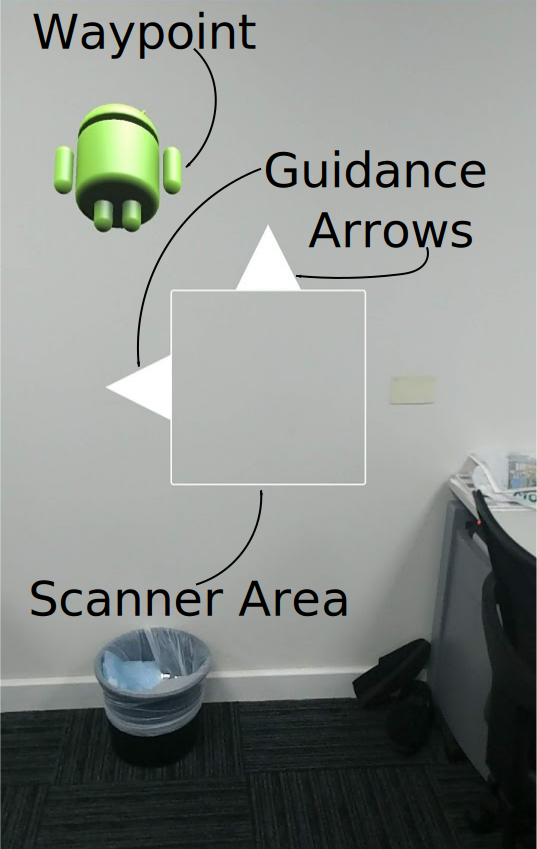
\includegraphics[width=0.3\textwidth]{figures/system_screenshot.png}
  \caption{A screenshot of the guidance interface showing a waypoint (based on an 3D Android model), the object scanner area and the guidance instruction arrows. }\label{fig:system-screenshot}
\end{figure}

The next section discusses other relevant work done in this field, followed by a detailed discussion on the design of the guidance system and MDP\@. Then we discuss the experiment and present its results, after which we conclude the paper and discuss the project's next steps. 

\section{\uppercase{Previous Work}}

\noindent Assistive vision and guidance for the VI is an active and diverse field of study. In recent years, the increase in mobile processing power and computer vision improvements have led to researchers investigating using a cellphone camera to augment or enhance a user's vision and help them find objects or another point of interest. Earlier attempts at the problem involved placing special markers or barcodes, encoded with information about an object or the area, around an environment, which the user then scans with a cellphone or similar mobile device~\cite{gude2013blind,iannizzotto2005badge3d,manduchi2012mobile}. This device then uses some feedback mode, e.g.\ Braille and sound, to guide the user towards the target. The major drawbacks to this approach is the significant upfront effort required to augment entire areas with markers to a point where the system will be useful to a VI user. Furthermore, these passive systems rely on the user scanning the marker in the first place; something that can be made more complicated with markers degrading over time, changing ambient lighting, different viewing angles and marker occlusion. 

Another approach is to discard tags completely and rely on computer vision to perform the object detection, something that has become more plausible with recent improvements to feature detectors and deep networks~\cite{huang2017speed,redmon2016you}. The system described~\cite{schauerte2012assistive} uses a combination of Scale Invariant Feature Transform (SIFT)~\cite{lowe1999object} and Speeded Up Robust Features (SURF)~\cite{bay2006surf} to detect known objects when they are in the camera's view and guide the user to them using sonified guidance instructions. This system is more flexible than the tag-based ones, but have the same drawback of being passive and rely on chance for the user to place the object within the camera's view in the first place. The paper also does not report on any performance metrics. In~\cite{bigham2010vizwiz}, the authors discuss their VizWiz system that offloads the object recognition tasks to an Amazon Mechanical Turk worker that then provides feedback on where the object of interest is located relative to the user. The VizWiz has the advantage of being fairly robust and is able to classify a great deal of objects with little effort from the user and can provide natural, human-generated and curated directions. However, this approach does not address the issue of enhancing user independence, since the user is now beholden to an online worker instead of a relative, friend or bystander. Furthermore, a good internet connection is required on the device, perhaps limiting use in some poor-reception areas.

As shown here, much research has been performed on object recognition and guidance towards an object once detected. However, work on active object search is harder to come by. Therefore, in this work we attempt to implement a system that uses active vision~\cite{aloimonos1988active} to guide a user towards an out-of-view target object by using the history of past object observations made during the search. With this, we hope to make the searching process less random and move towards a more natural search object searching process. 

\section{\uppercase{Guidance System Design}}

\noindent The guidance system is built into an Android app with Android's ARCore~\footnote{https://developers.google.com/ar/} API enabled and is designed with the goal of generating a path of waypoints for the user to follow with a camera that will lead to the target object. This path is generated one waypoint at a time by the system and is updated with every object observation the user makes when adjusting the camera. We modelled this optimal path search problem as a grid-world problem that is solved by an Markov Decision Process (MDP) model. The details of the grid layout and the MDP model are discussed in the sections below. For this initial design, the system only works in the pan and tilt dimension and the depth dimension will be added after successful testing of this version of the guidance system.

\subsection{Environment Design}\label{sec:env-design}

\noindent We model this problem on the familiar grid-world problem, where an agent is tasked move to a terminal square from an origin square given some constraints. However, instead of the traditional, linear grid-world problem, we use the grid in a radial coordinate system which surrounds the user and each grid square represent a pan/tilt angle coordinate. See Fig.~\ref{fig:environment} for an example grid. Since we do not consider the depth dimension yet, each grid square is equidistant from the user and agent. The agent translates between the squares as the user points the camera in different directions.

\begin{figure}  
  \centering
  \input{figures/fig.tex}
\caption{A diagram of the radial grid-world used in the MDP is modelled with. }\label{fig:environment}
\end{figure}

MDPs are well-suited to solving this class of problem, i.e.\ to find the optimal route from the origin square to the terminal square, so modelling our problem as a grid-world allows us to design our guidance system and MDP model with existing and well-understood models and techniques. Each square of the grid represents a combination of the agent's pan-tilt-observation, or state, which is discussed in more detail in Sec.~\ref{sec:states}. The terminal square is the square whose state contains the target object, or observation. The grid size can be adjusted to control the model's resolution: smaller squares will increase accuracy, but at the cost of performance, both during use (more squares need to be traversed) and training (much larger state space). For the initial system design, we set the grid resolution to \SI{30}{\degree}.

\subsection{MDP Design}

\noindent The MDP model was used to produce a policy that defines a set of optimal actions for the agent to take in any given state. In this case, the agent is defined as the mobile phone and guidance system and the policy is used to generate the next waypoint on the search path towards the square on the grid that contains the target object. We initially assume perfect state and transition observability for each timestep and once we have a better understanding of the sensor limitations, we can expand the problem to a more sophisticated, and perhaps more representative, Partially Observable MDP (POMDP) problem. For now, the problem is given by the 5-tuple

\begin{equation}
  <\mathbf{S}, \mathbf{A}, \mathbf{T}, \mathbf{R}, \gamma>, 
\end{equation}
where $\mathbf{S}$ is a set of possible states the agent can be in, $\mathbf{A}$ is a set of possible actions an agent can take in any given state, $\mathbf{T}$, is a set of state transition probabilities defining the probability of transitioning from state $s$ to state $s'$. $\mathbf{R}$ is the reward function defining the immediate reward the agent receives from executing an action $a$ in state $s$, and $\gamma$ is a discount factor which represents the models priority in maximising immediate rewards over long-term reward. Each of these elements are defined and discussed here.

\subsubsection{States}\label{sec:states}

\noindent The state is a combination of different trackable parameters that the agent may possess at any given time that defines the agent's decision process. The agent's state vector is given by 

\begin{equation}
  \mathbf{S} = s(o, n, s), 
\end{equation}
where $o$ is the current observation, $n$ is the number of steps taken during the search and $s$ is a binary variable that tracks whether a pan/tilt position has been visited before during the search. There are 8 observations encoded into the system, including a `nothing' observation where nothing of note is observed, and they are also the possible targets. For an initial implementation, we are simulating a simple office and we selected the possible objects as objects one might typically expect to see in a normal office. These objects are

\begin{equation}
  \begin{aligned}
    o\in \{monitor, mouse, keyboard, window, mug,\\ office\;supplies, desk, nothing\}.
  \end{aligned}
\end{equation}

The model tracks a total of 12 steps to the target. We select 12 since the longest route one could take between the furthest corners on the 6$\times$6 grid we used is 12. The MDP therefore has a total of 216 possible states ($8\times12\times2$).

\subsubsection{Actions}

The policy produced by an MDP define the action an agent will take when it finds itself in any given state. In this case, the action is the direction the user should move towards in a grid-world context, i.e.\ the angular adjustment the user must make to the camera to move along the search path. This action is interpreted by the guidance system and a new waypoint is added to the search path toward the target object. The action is defined by

\begin{equation}
  \mathbf{A} = a(s),
\end{equation}
and the possible actions are

\begin{equation}
  a\in \{UP, DOWN, LEFT, RIGHT\}.
\end{equation}

The number of actions can of course be expanded to increase resolution, but for this experiment and grid setup, they are sufficient. 

\subsubsection{State Transition Probabilities}

\noindent The state transition function, $\mathbf{T}$, defines the likelihood of the agent transitioning into a state $s'$ from state $s$ when taking an action $a$, i.e.\ the likelihood of moving into a square and making observation $o$ after performing action $a$. It therefore contains the spatial relationships between the different objects in the observation set. Formally, the transition function is defined by

\begin{equation}
  T(s, a, s') = t.
\end{equation}

The spatial relationships are extracted from Google's OpenImage dataset\footnote{https://storage.googleapis.com/openimages/web/index.html}~\cite{openimages}. This dataset consists of 1.74M images containing 14.6M labelled bounding boxes manually drawn around objects and is primarily aimed toward object recognition researchers to test their models on. However, with the bounding boxes and object labels we can extract the spatial relationships between the different objects in our observation set. Since the camera perspectives and absolute distances between the objects in the images aren't given, we can only extract the relationships in simple terms with little context, e.g.\ we can only say that object 1 is above object 2, but not how far above. Our simple action-space and grid environment somewhat compensates for this lack of complexity in the dataset. 

\subsubsection{Reward Function}

\noindent The reward function, $\mathbf{R}$, is the immediate reward that the agent receives after transitioning from state $s$ to state $s'$ and is given by 

\begin{equation}
  \mathbf{R} = r(s, s').
\end{equation} 
This is an important parameter for training the agent to produce the most effective policy. 

During training, we define a negative reward for exceeding the 12-step limit we defined in the model, as well as if it re-enters a previous search location. Conversely, the agent is given a significant reward when it finds the target object. The goal of the agent is to maximise its cumulative reward over time. These numbers are chosen such that they motivate the agent to reach the target, while hastening the process by punishing it every time it re-explores a state and the longer it takes to reach the target. 

\subsubsection{Model Training}

\noindent The policy is generated through a training process where the agent is placed in an environment with some constraints and attempts to maximise its short- and long-term reward through interacting with the environment. This problem is solved as an optimisation problem, where the agent will potentially start with a very inefficient, or wholly ineffective, policy and over time and many iterations, improve its policy and reach the target in an optimum number of timesteps. 

The training environment is a simple mathematical representation of the grid-world described in Sec.~\ref{sec:env-design} that have the following constraints during training to optimise the agent's search strategy:

\begin{itemize}
  \item the agent must face forward, i.e.\ viewing angle must be less than \SI{90}{\degree} from the vertical and horizontal planes,
  \item the agent can only move one square (angle interval) at a time, 
  \item the process terminates when the target object is observed,
\end{itemize}

The lack of absolute spatial information in the OpenImage dataset made the data seem fairly ambiguous in some cases, which makes it hard to find a single, optimal solution to the problem. We therefore could not use the popular value iteration algorithm~\cite{bellman1957markovian} and opted for the state-action-reward-state-action (SARSA) algorithm~\cite{rummery1994line} instead. SARSA is an on-policy algorithm with the advantage of being more exploratory in nature and is therefore more likely to find a solution. However, this solution is not guaranteed to be optimal, but can get very close to the optimal solution. This is a fairly simple MDP with a relatively small state-action-observation space, which makes it possible to find a solution in a reasonable amount of time. However, it should be noted that adjusting the angle interval or adding more actions or observations can easily blow up the size of the state-space. 

\section{\uppercase{Experiments}}

\noindent To test the effectiveness of the policy the MDP produced, we designed a set of experiments that determined how effective the system is at directing a participant to pointing towards a target object. This section discusses all of the simulations and experiments that were carried out. 

\subsection{Experiment Design}

\noindent To test the viability and effectiveness of our system, we carried out a set of experiments. For this, the MDP policies were integrated into an Android application that uses the camera to provide observation data and track the pose and viewing direction. We avoided adding unnecessary variability and complexity to the experiment by providing visual waypoints on screen which the participants were allowed to use. In addition to this, encoded QR codes and the Android barcode scanner library were used to simulate object detection. A generic environment mimicking a typical office desk layout was set up as the experiment environment and contains 7 different objects (i.e.\ encoded QR codes), one of which were the target object. See Figure~\ref{fig:env-picture} for a picture of the environment. 

\begin{figure}
  \centering
  \includegraphics[width=0.4\textwidth]{figures/test_env_picture.jpg}
  \caption{A picture of the environment used for the experiments. Each QR code represents an object. }\label{fig:env-picture}
\end{figure}

For each experiment, the participant was placed roughly \SI{1}{\meter} from the barcodes and was asked not to move from that spot during the experiment. The participant then pressed a button on the app that randomly selected a target object and was then guided towards that target by the app. Since the participants were allowed to use their vision, the targets were randomly selected and the participants were uninformed of what the target object was until it was found. This was done to avoid the participants learning the target objects' locations between each search run.

During in-house tests, we noted that the system sometimes makes guidance mistakes that lead the user towards the edge of the search space, at which point the system had difficulty guiding the user back to the centre. To avoid this having an adverse impact and drawing out the experiments too long, we set a search step limit of 16, which means that only 16 waypoints were be generated before the search was terminated. A search run therefore ended when the participant either successfully found the target object by pointing the phone camera to it and scanning the barcode, or exceeded the waypoint limit. After this, the participant then resets to the central position, selects a new target object and resumes the experiment.

The participants were left to repeat this process until we recorded 10 searches per object, giving us a total number of 70 recorded search samples per participant. We tested a total of 10 different participants (sex: 8 M, 2 F;\@ age: $\mu$ 31.2 years, $\sigma$ 8 years), most of which were sourced from our laboratory with none having any disabilities or handicaps. This gives our dataset a total of 700 search samples.

\subsection{Results}

\noindent In order to evaluate our system, we identified 3 different measures: target acquisition rate (TAR), number of steps to the target and the total time it took to find a target object. We present and discuss the results for each of these parameters in the next sections. All of the results are summarised in Table~\ref{tab:results-summary}.

\begin{table}
  \centering
  \caption{A table containing a summary of the TAR, steps and time to target means ($\mu$) and standard deviations ($\sigma$) for each individual participant and the entire participant population.}\label{tab:results-summary}
  \begin{tabular}{cc|cc|cc}
    \toprule
    \multirow{2}{*}{Participant} & \multirow{2}{*}{TAR [\%]} & \multicolumn{2}{c|}{Num. Steps} & \multicolumn{2}{c}{Time [s]} \\ 
				 &			     & $\mu$ & $\sigma$		       & $\mu$ & $\sigma$  \\ \midrule
    s1 & 6.3 & 7.2 & 5.4 & 29 & 22 \\ \midrule
    s2 & 21 & 6.7 & 4.8 & 34 & 5.1 \\ \midrule
    s3 & 8.8 & 6.3 & 4.9 & 31 & 21 \\ \midrule
    s4 & 21 & 6.7 & 4.3 & 37 & 5.6 \\ \midrule
    s5 & 24 & 7.2 & 4.9 & 33 & 14 \\ \midrule
    s6 & 40 & 8.2 & 5.4 & 24 & 10 \\ \midrule
    s7 & 14 & 8.5 & 5.8 & 31 & 16 \\ \midrule
    s8 & 12 & 5.1 & 4.0 & 39 & 21 \\ \midrule
    s9 & 2.5 & 7.2 & 5.4 & 39 & 18 \\ \midrule
    s10 & 33 & 6.6 & 5.4 & 26 & 12 \\ \midrule\midrule
    Population & $\mu$: 18 $\sigma$: 11 & 6.8 & 5.1 & 34 & 23 \\
    \bottomrule
  \end{tabular}
\end{table}

\subsection{Target Acquisition Rate}

\noindent The target acquisition rate (TAR) is a measure of how successful the system was at directing a participant to the target object within the 16-step limit we imposed and is simply calculated as a proportion of the number completed searches vs.\ the total number of searches. See Figure~\ref{fig:incomplete-searches-subjects} for a plot showing the TAR for each participant. Please note, however, that this plot is dependant on the step-limit we selected and should not be taken as an absolute measure of performance, but is rather presented to provide context to the other results we present. 

\begin{figure}
  \centering
  \includegraphics[width=0.5\textwidth]{figures/incomplete_searches_subjects.png}
  \caption{A plot giving the proportion of searches that reached the 16-step limit we imposed for each participant. }\label{fig:incomplete-searches-subjects}
\end{figure}

The inter-participant spread ($\sigma=11\%$) is fairly significant, perhaps indicating that the user's search behaviour and strategy affects the target acquisition performance  With an average TAR of $18.3\%$, it is clear that our system can be improved with regards to entering a no-recovery state where it directs a user into dead-space with no spatial information (e.g.\ a ceiling or wall section) and cannot gather the information it requires to intelligently guide the user. Subsequent system updates will have to consider implementing fall-back methods or other automatic recovery modes that can detect entry of a no-recovery state (e.g.\ exceeding a set number of steps/time without making an observation) and guide the user back to the initial position.

\subsection{Number of Steps to Target}

\noindent The number of steps to target indicates the number of waypoints the system generated for the participant during the guidance process is a major indication of system performance, where less waypoints means better performance. Figure~\ref{fig:nsteps-participants} shows the distributions of the number of steps to the target for each individual participant. 

\begin{figure}
  \centering
  \includegraphics[width=0.5\textwidth]{figures/boxplot_nsteps_subjects.png}
  \caption{The distributions of each participant's number of steps taken to find a target object. }\label{fig:nsteps-participants}
\end{figure}

The number of waypoints each participant required is fairly consistent across all of the participants with a inter-participant standard deviation of 1 waypoint. The population mean and standard deviation is 6.8 and 5.1 waypoints respectively. This is a reasonable result that was also somewhat expected, since most target objects were placed within approximately 4 grid squares away from the participants' initial looking directions.

It is interesting to note that participants $s6$ and $s10$ also found their targets within these reasonable bounds when accounted for the targets that they found within the 16-step limit. This supports the argument from the previous results that their decreased TAR was partly caused by an abnormally high number of entries into a no-recovery state and further reinforces the need to implement an automatic recovery feature in the system before deployment. 

\subsection{Time to Target}

\noindent The total time it took a participant to reach the target object is given in Figure~\ref{fig:time-participants}. In it we see that the inter-participant variance in the temporal response, with mean 29.8s and standard deviation 6.2s (population standard deviation of 23s), is far greater than for the number of waypoints they required. Indeed, there is not a strong relationship between the number of waypoints a participant required and the time they took to find the target, as showcased by participant $s7$'s wide mean waypoint count and spread in Figure~\ref{fig:nsteps-participants} and the small spread and close-to-average time to target in Figure~\ref{fig:time-participants}. Furthermore, the opposite can be observed in participant $s8$'s small spread and low mean waypoint count in Figure~\ref{fig:nsteps-participants} and high spread and high mean time to target in Figure~\ref{fig:time-participants}. 

\begin{figure}
  \centering
  \includegraphics[width=0.5\textwidth]{figures/boxplot_time_to_target_subjects.png}
  \caption{The distributions of the each participant's time taken to find a target object. }\label{fig:time-participants}
\end{figure}

In comparison to the VizWiz system~\cite{bigham2010vizwiz} (mean 92s, standard deviation 37.7s), our results look fairly reasonable. However, our results may look very different when we test the system with VI participants like they did in~\cite{bigham2010vizwiz}.

\section{\uppercase{Future Work and Conclusion}}

\noindent In this work we presented and tested an MDP-based system to guide a visually impaired (VI) person towards a target object with no apriori knowledge of the environment. We implemented the system in an Android app that we tested with a small group of sighted people to determine its viability and effectiveness at guiding user at finding and pointing a camera at a specific target. We found that is works fairly well when compared to alternative systems, with a respectable mean time of target acquisition of 32s. However, the system can be improved by refining the search strategy and implementing an automatic fail-state recovery system that will guide a user back to neutral position if a fail-state is entered (e.g.\ a blank section of wall). 

The next steps to this project will involve using the data recorded here to improve and refine the MDP model that provides the guidance. The model can also be expanded to include more objects and actions. However, an important consideration and expansion to the problem is to change the MDP to an Partially Observable MDP (POMDP) that will bring the model more in line with reality by acknowledging that the objects are not perfectly observable and humans do not perfectly follow guidance instructions. This adjustment may be very important when we consider that we will replace the QR code detector with object recognition models that are typically more prone to making classification errors. Finally, the model can be adapted to use on-line learning techniques in order to further refine its transition model as the user uses the guidance system. 

\clearpage
\bibliographystyle{apalike}
\bibliography{bib}

\end{document}
